
\documentclass[11pt,a4paper]{article}
\usepackage[utf8]{inputenc}
\usepackage[T1]{fontenc}
\usepackage[spanish,es-nodecimaldot]{babel}
\usepackage[a4paper,left=1.7cm,right=1.7cm,top=20mm,bottom=20mm]{geometry}
\usepackage{amsmath,amssymb,amsfonts,mathtools,bm}
\usepackage{braket}
\usepackage{graphicx}
\usepackage{float}
\usepackage{booktabs}
\usepackage{enumitem}
\usepackage{xcolor}
\usepackage{lmodern,microtype}
\usepackage{fancyhdr}
\usepackage{titlesec}
\usepackage[colorlinks=true,linkcolor=black,urlcolor=black,citecolor=black]{hyperref}
\numberwithin{equation}{section}
\renewcommand{\boxed}[1]{#1}
\setlength{\parindent}{0pt}
\setlength{\parskip}{5pt}
\newcommand{\dd}{\,\mathrm d}
\newcommand{\ii}{\mathrm i}
\newcommand{\e}{\mathrm e}
\newcommand{\hb}{\hbar}
\newcommand{\R}{\mathbb R}
\newcommand{\C}{\mathbb C}
\newcommand{\id}{\mathbb I}

\pagestyle{fancy}
\setlength{\headheight}{14pt}
\fancyhf{}
\fancyhead[L]{\textit{Tarea 2}}
\fancyhead[R]{Física VII: Introducción a la Mecánica Cuántica}
\begin{document}
\begin{titlepage}
\centering
\vspace*{1.8cm}

\includegraphics[width=.22\textwidth]{UdeC_escudo.png}
\vspace{1.1cm}

{\Huge\bfseries Tarea 2\par}
\vspace{.4cm}
{\Huge\bfseries Física VII: Introducción a la Mecánica Cuántica\par}
\vspace{1.5cm}
{\Large José Ignacio Rosas Sepúlveda\par}
\vspace{.8cm}
{\Large Solución\par}
\vfill
\thispagestyle{empty}
\end{titlepage}
\tableofcontents
\newpage
\section*{Enunciado}
\addcontentsline{toc}{section}{Enunciado}
\begin{enumerate}[label=\arabic*.-]
\item Considere una partícula de energía $E>V_0$ en movimiento unidimensional, que incide desde la izquierda sobre un escalón descendente situado en $x=0$,
\begin{equation}
V(x)=\begin{cases}V_0,&x<0,\\0,&x>0,\end{cases}
\qquad V_0>0.
\end{equation}
\begin{enumerate}[label=\alph*)]
\item Encuentre el coeficiente de transmisión $T$.
\item Grafique $T$ como función de $E/V_0$.
\item Comente el resultado comparándolo con el comportamiento de una partícula clásica.
\end{enumerate}

\item Considere una partícula que incide desde la izquierda con energía $E$ sobre la barrera delta
\begin{equation}
V(x)=\alpha\,\delta(x),\qquad \alpha>0,
\end{equation}
donde $\alpha$ tiene unidades de J\,m.
\begin{enumerate}[label=\alph*)]
\item Demuestre que $\psi'(x)$ es discontinua en $x=0$ y que
\begin{equation}
\psi'_{II}(0)-\psi'_I(0)=\frac{2m\alpha}{\hbar^2}\psi(0).
\end{equation}
\item Para
\begin{align}
\psi_I(x,t)&=\left(A_+e^{ikx}+A_-e^{-ikx}\right)e^{-iEt/\hbar},\qquad x<0,\\
\psi_{II}(x,t)&=B_+e^{ikx}e^{-iEt/\hbar},\qquad x>0,
\end{align}
con $k=\sqrt{2mE}/\hbar$, use la discontinuidad anterior y la continuidad de $\psi$ para calcular $T$ y $R$.
\item Grafique $T$ y $R$ como funciones de $\mathcal E=E/(m\alpha^2/2\hbar^2)$.
\item Demuestre que para $E\gg m\alpha^2/(2\hbar^2)$ se tiene $T\to1$ y comente el resultado comparándolo con el caso clásico.
\end{enumerate}

\item Considere el pozo delta atractivo
\begin{equation}
V(x)=-\alpha\,\delta(x),\qquad \alpha>0.
\end{equation}
\begin{enumerate}[label=\alph*)]
\item Demuestre que una partícula confinada en el pozo sólo puede tener un valor propio de energía dado por $E=-2m\alpha^2/\hbar^2$.
\item Encuentre la correspondiente función de onda propia normalizada.
\end{enumerate}
\end{enumerate}
En lo posible, comente sus resultados en cada una de las preguntas.


\section{Problema 1}
Para una onda plana $D e^{ikx}$ la corriente de probabilidad es $j=(\hbar k/m)|D|^2$. Usaremos esta expresión, tal como en la clase, para definir transmisión y reflexión mediante cocientes de corrientes.

Sea
\begin{equation}
V(x)=\begin{cases}V_0,&x<0,\\0,&x>0,\end{cases}\qquad E>V_0,
\end{equation}
y definamos
\begin{equation}
k_1=\frac{\sqrt{2m(E-V_0)}}{\hb},\qquad
k_2=\frac{\sqrt{2mE}}{\hb}.
\end{equation}
Para incidencia desde la izquierda,
\begin{equation}
\psi_I=A\e^{\ii k_1x}+B\e^{-\ii k_1x},\qquad
\psi_{II}=C\e^{\ii k_2x}.
\end{equation}
Como el potencial es finito en $x=0$, tanto $\psi$ como $\psi'$ son continuas. Por tanto,
\begin{equation}
A+B=C,\qquad k_1(A-B)=k_2C.
\end{equation}
Eliminando $B$ entre ambas ecuaciones,
\begin{align}
A-B&=\frac{k_2}{k_1}C,\\
2A&=C\left(1+\frac{k_2}{k_1}\right),
\end{align}
y, por tanto,
\begin{equation}
\frac{C}{A}=\frac{2k_1}{k_1+k_2},\qquad
\frac{B}{A}=\frac{k_1-k_2}{k_1+k_2}.
\end{equation}
El flujo de probabilidad de una onda $D\e^{\ii kx}$ es $j=\hb k|D|^2/m$. Por tanto,
\begin{equation}
\boxed{T=\frac{k_2}{k_1}\left|\frac{C}{A}\right|^2
=\frac{4k_1k_2}{(k_1+k_2)^2}.}
\end{equation}
En función de $\varepsilon=E/V_0$,
\begin{equation}
T(\varepsilon)=\frac{4\sqrt{\varepsilon(\varepsilon-1)}}{
(\sqrt{\varepsilon}+\sqrt{\varepsilon-1})^2},\qquad \varepsilon>1.
\end{equation}
\begin{figure}[H]\centering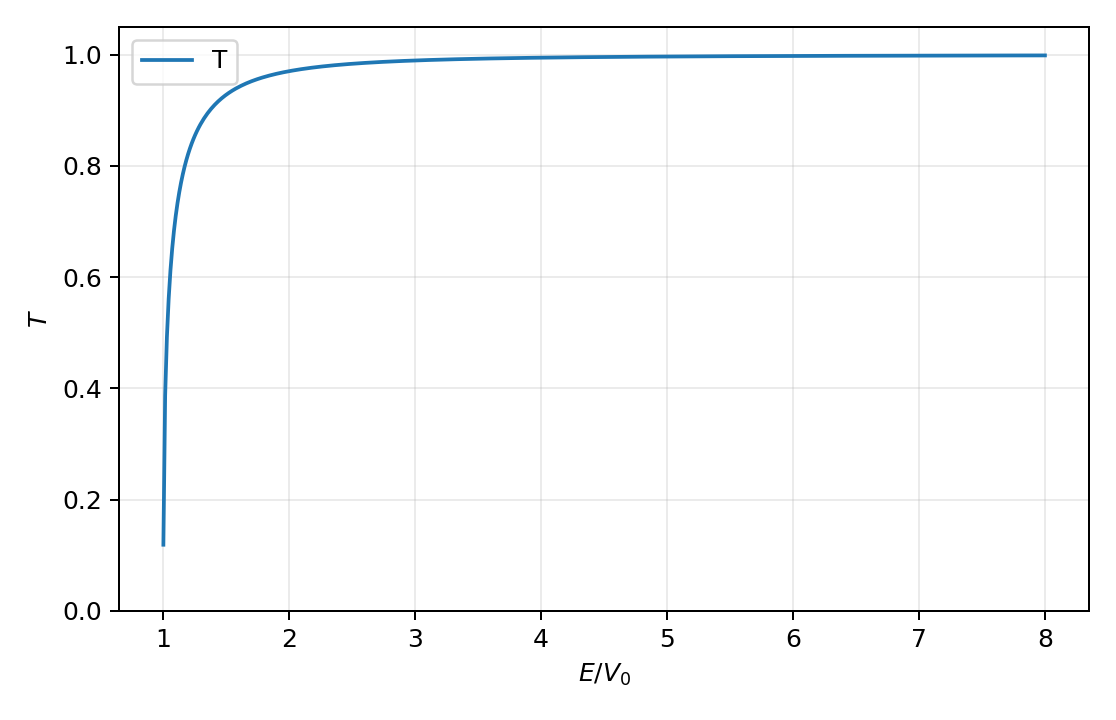
\includegraphics[width=.68\textwidth]{figures/escalon_transmision.png}\caption{Transmisión por un escalón descendente.}\end{figure}

\paragraph{Comentario.}
Clásicamente, si $E>V_0$ la partícula atraviesa siempre el escalón: $T_{\rm cl}=1$. Cuánticamente existe reflexión aun cuando no hay región clásicamente prohibida. Esa reflexión desaparece gradualmente cuando $E\gg V_0$.


\section{Problema 2}
La delta de Dirac se usa en el sentido distributivo, $\int\delta(x)f(x)\,\mathrm dx=f(0)$. Esta propiedad permite obtener la condición que reemplaza a la continuidad de $\psi'$.

Sea $V(x)=\alpha\delta(x)$ con $\alpha>0$. Integramos la ecuación de Schrödinger estacionaria entre $-\epsilon$ y $+\epsilon$:
\begin{equation}
-\frac{\hb^2}{2m}\int_{-\epsilon}^{\epsilon}\psi''\dd x
+\alpha\int_{-\epsilon}^{\epsilon}\delta(x)\psi(x)\dd x
=E\int_{-\epsilon}^{\epsilon}\psi\dd x.
\end{equation}
Si $\psi$ permanece acotada, $\int_{-\epsilon}^{\epsilon}\psi\,\mathrm dx\to0$ cuando $\epsilon\to0$. En cambio, la integral con la delta conserva el valor $\psi(0)$. Así,
\begin{equation}
-\frac{\hbar^2}{2m}\left[\psi'(0^+)-\psi'(0^-)\right]+\alpha\psi(0)=0,
\end{equation}
y resulta
\begin{equation}
\boxed{\psi'(0^+)-\psi'(0^-)=\frac{2m\alpha}{\hb^2}\psi(0).}
\end{equation}
La propia función de onda permanece continua. Escribimos
\begin{equation}
\psi_I=A\e^{\ii kx}+B\e^{-\ii kx},\qquad
\psi_{II}=C\e^{\ii kx},\qquad k=\frac{\sqrt{2mE}}{\hb}.
\end{equation}
La continuidad da $A+B=C$. La condición de salto da
\begin{equation}
ikC-ik(A-B)=\frac{2m\alpha}{\hbar^2}C.
\end{equation}
Usando $B=C-A$ y definiendo $\gamma=m\alpha/(\hbar^2k)$, se obtiene
\begin{equation}
t\equiv\frac{C}{A}=\frac{1}{1+\ii\gamma},\qquad
r\equiv\frac{B}{A}=\frac{-\ii\gamma}{1+\ii\gamma}.
\end{equation}
Como ambos lados tienen el mismo $k$,
\begin{equation}
\boxed{T=\frac{1}{1+\gamma^2},\qquad R=\frac{\gamma^2}{1+\gamma^2},\qquad T+R=1.}
\end{equation}
Con $E_\alpha=m\alpha^2/(2\hb^2)$ y $\epsilon=E/E_\alpha$,
\begin{equation}
\boxed{T=\frac{\epsilon}{1+\epsilon},\qquad R=\frac{1}{1+\epsilon}.}
\end{equation}
\begin{figure}[H]\centering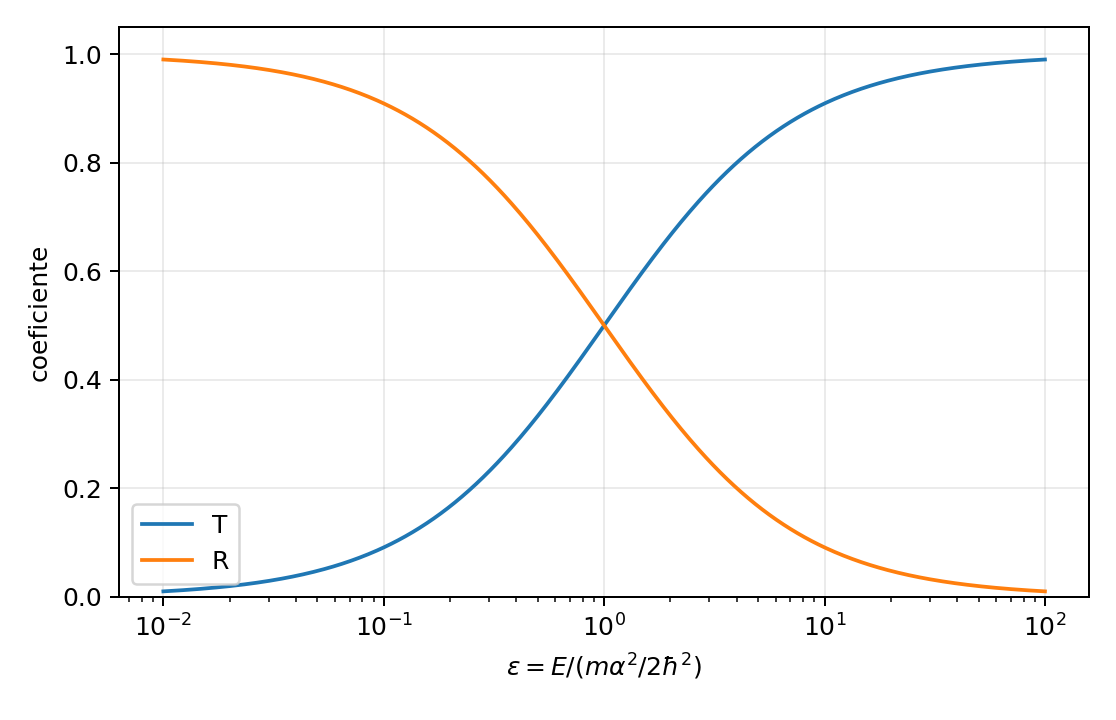
\includegraphics[width=.68\textwidth]{figures/delta_TR.png}\caption{Transmisión y reflexión para la barrera delta.}\end{figure}
Para $E\gg E_\alpha$, $T\to1$. El resultado expresa el límite de correspondencia: una partícula suficientemente energética es apenas afectada por una barrera localizada.

\section{Problema 3}
Ahora $V(x)=-\alpha\delta(x)$, con $\alpha>0$. Para un estado ligado escribimos
\begin{equation}
E=-\frac{\hb^2\kappa^2}{2m},\qquad \kappa>0.
\end{equation}
La normalizabilidad exige
\begin{equation}
\psi(x)=A\e^{-\kappa|x|}.
\end{equation}
La condición de salto cambia de signo:
\begin{equation}
\psi'(0^+)-\psi'(0^-)=-\frac{2m\alpha}{\hb^2}\psi(0).
\end{equation}
La continuidad en $x=0$ fija la misma constante a ambos lados. Además,
\begin{equation}
\psi'(0^+)=-\kappa A,\qquad \psi'(0^-)=+\kappa A.
\end{equation}
Por ello,
\begin{equation}
-2\kappa A=-\frac{2m\alpha}{\hb^2}A,
\qquad
\kappa=\frac{m\alpha}{\hb^2}.
\end{equation}
Por tanto,
\begin{equation}
\boxed{E=-\frac{m\alpha^2}{2\hb^2},\qquad
\psi(x)=\sqrt{\frac{m\alpha}{\hb^2}}\exp\left[-\frac{m\alpha}{\hb^2}|x|\right].}
\end{equation}

\paragraph{Corrección física del enunciado.}
La energía $-2m\alpha^2/\hb^2$ que aparece en el apunte no satisface simultáneamente la ecuación de Schrödinger y la condición de salto. El cálculo directo fija de manera unívoca el factor $1/2$ mostrado arriba.



\end{document}
